卟啉的英文名``porphyrin''源自于古希腊词汇``\emph{porphyra}'',意为紫色。卟啉是一系列大环有机化合物的总称,其中包含四个被修饰的吡咯单元。卟啉共有26个$\pi$电子,其中18个构成了平面的卟啉环结构,常被认为具有芳香性。在自然界中,存在着卟啉与金属的配合物,其中最广为人知的一族卟啉配合物是红细胞色素,亚铁血红素。苯并卟啉由苯环与卟啉环中的吡咯单元邻接而成。

\begin{figure}[h!]
	\centering
	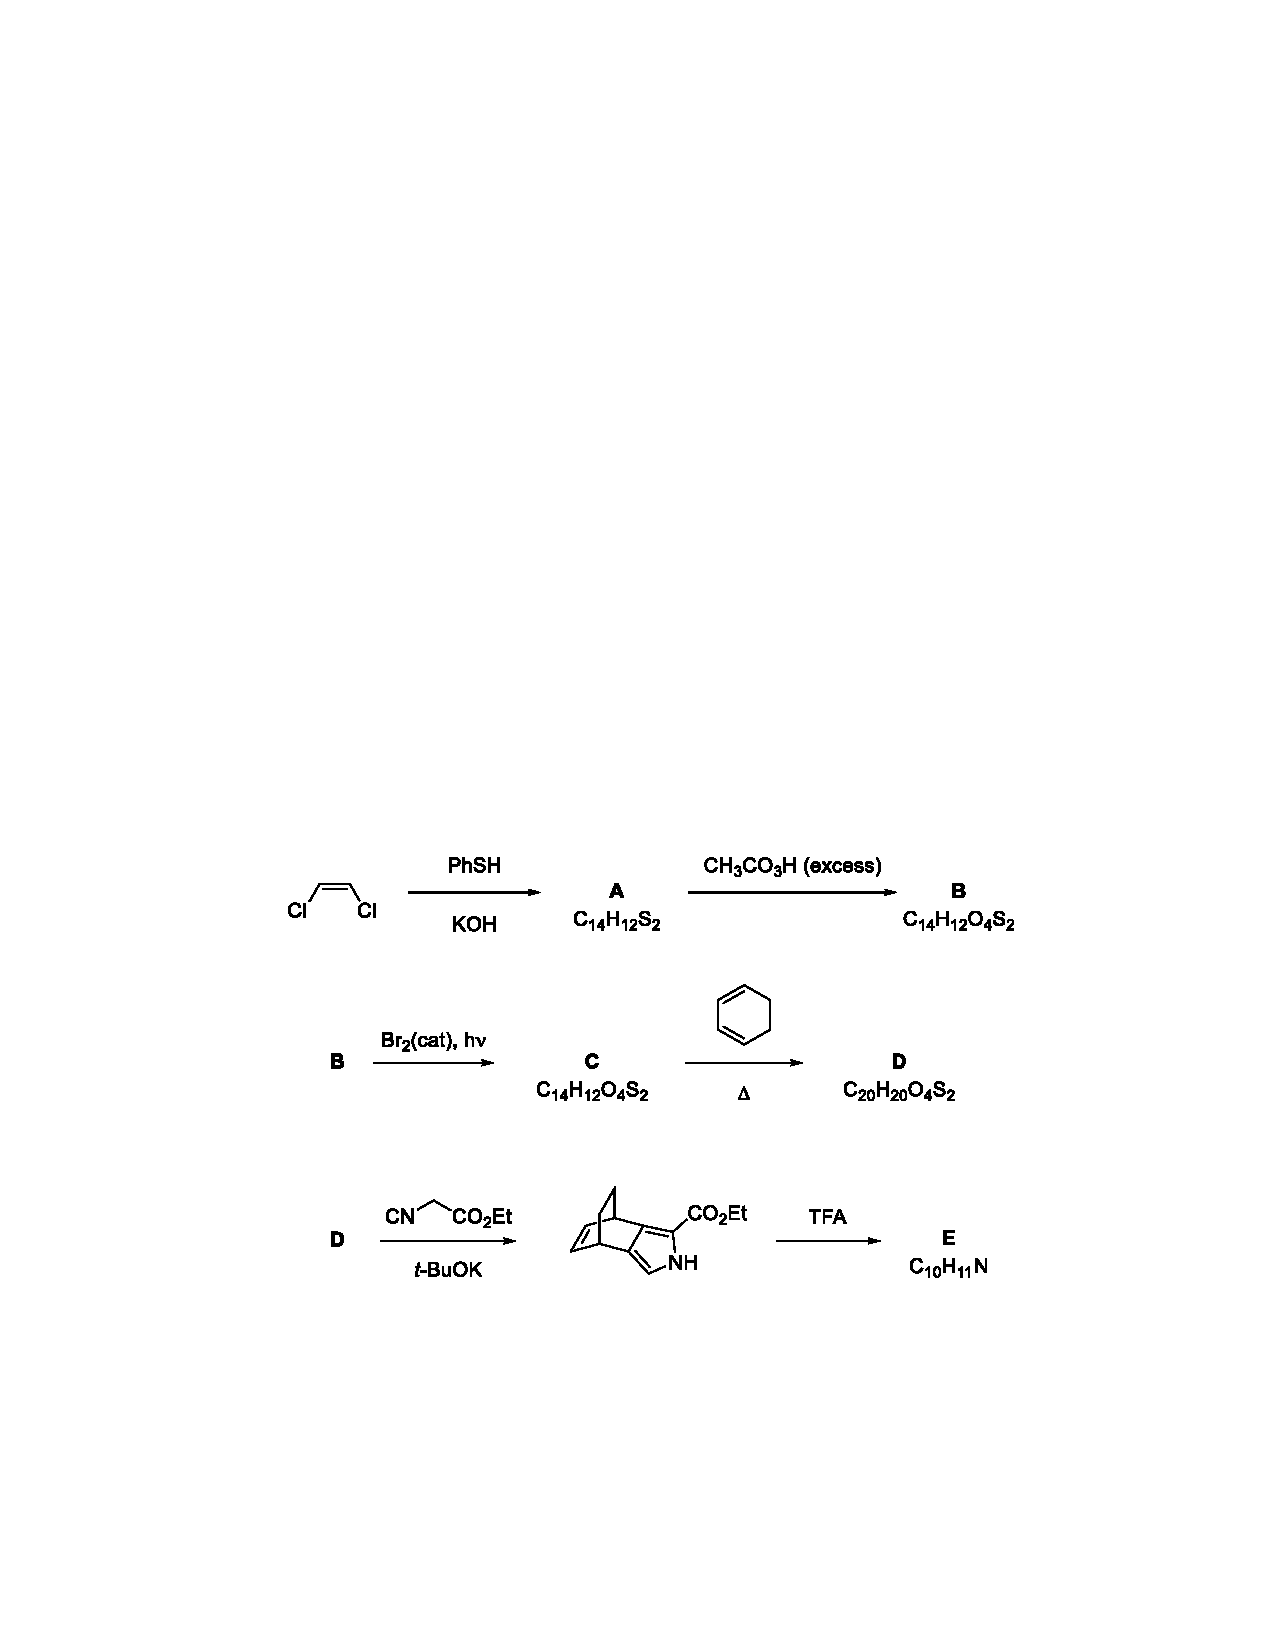
\includegraphics[width=11cm]{./pic/t11-1.pdf}
\end{figure}

苯并卟啉可以由吡咯衍生物\textbf{E}制备,上面的合成路线展示了化合物\textbf{E}的制备方法。首先,反式1,2-二氯乙烯与苯硫酚反应生成化合物\textbf{A},化合物\textbf{A}经氧化生成化合物\textbf{B},化合物\textbf{B}带有苯磺酰单元。顺式化合物\textbf{B}在紫外光照射下经催化量的Br\textsubscript{2}处理转化为其反式异构体\textbf{C},\textbf{C}与1,3-环己二烯在加热条件下发生Diels-Alder反应得到化合物\textbf{D}。化合物\textbf{D}与异氰基乙酸乙酯反应生成一种吡咯甲酸酯衍生物,其与TFA反应生成吡咯衍生物\textbf{E}。

\begin{figure}[h!]
	\centering
	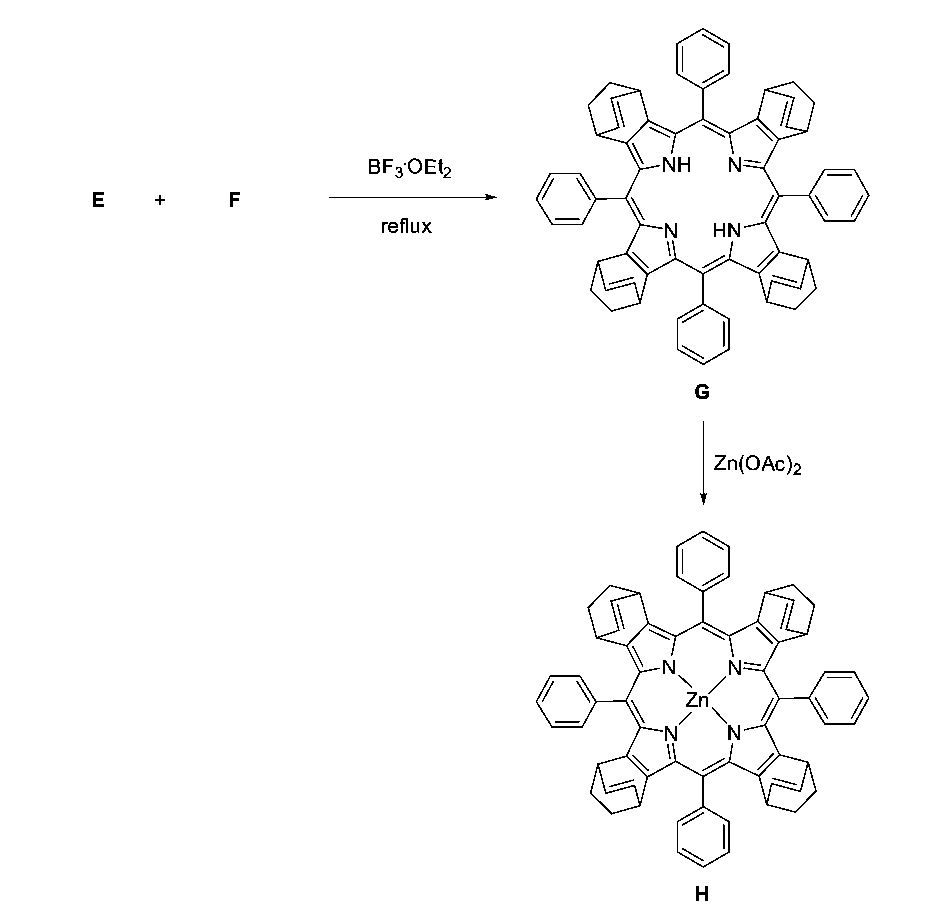
\includegraphics[width=12cm]{./pic/t11-2.pdf}
\end{figure}

\noindent\textbf{11.1.}画出化合物\textbf{A-E}的结构,必要时需表示出立体化学。

\noindent\textbf{11.2.}
卟啉可由吡咯衍生物与醛类化合物经环化反应制备。画出醛类化合物\textbf{F}的结构,写出化合物\textbf{H}中锌的氧化态。

将化合物\textbf{H}在真空中加热,它会发生逆Diels-Alder反应,生成一个共轭体系更大的化合物。

\noindent\textbf{11.3.} 在虚线圆圈内画出化合物\textbf{I}不全的部分,画出化合物\textbf{J}。

\begin{figure}[h]
	\centering
	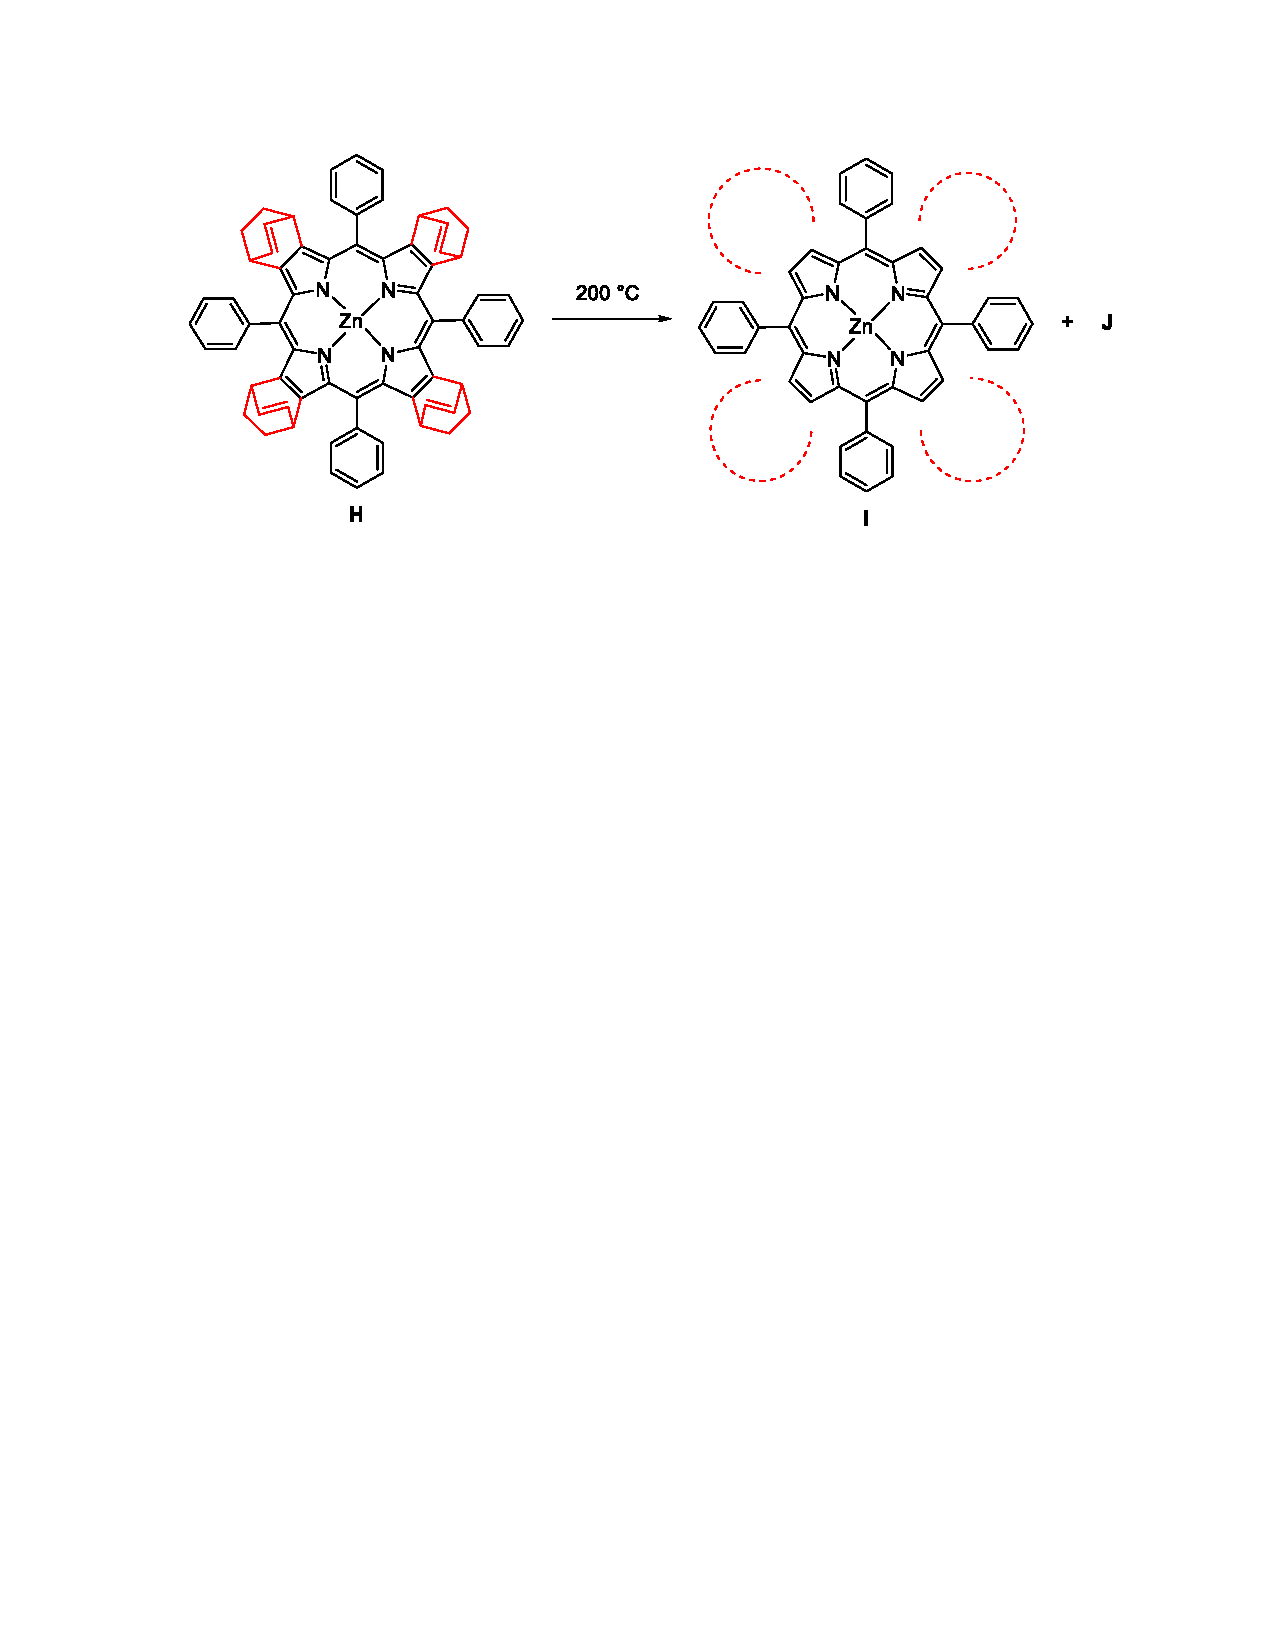
\includegraphics[width=13cm]{./pic/t11-3.pdf}
\end{figure}

氨是一种重要的参与新陈代谢的分子,由于其与某些特定疾病有关,关于如何灵敏而准确地测定其浓度的研究近来十分受重视。在正常生理条件下,弱碱性血液中的氨可通过皮肤或呼吸排出。肝脏、肾脏可将氨转化为尿素,在这两个器官功能紊乱时,呼吸和尿液中的氨浓度会升高,因此对呼吸和尿液中氨浓度的探测可作为鉴定早期肝脏和胃部疾病的指标。要达到此目标,需要发展灵敏度在50 ppb-2 ppm,响应迅速的测量传感器。

为此,化合物\textbf{I}被用于光纤氨分子探测传感器,氨分子能改变这种光纤的透光率。将不同浓度的氨气通过探测器,使用合适的光谱探测透光率的变化,结果列于下表。

\begin{figure}[h]
	\centering
	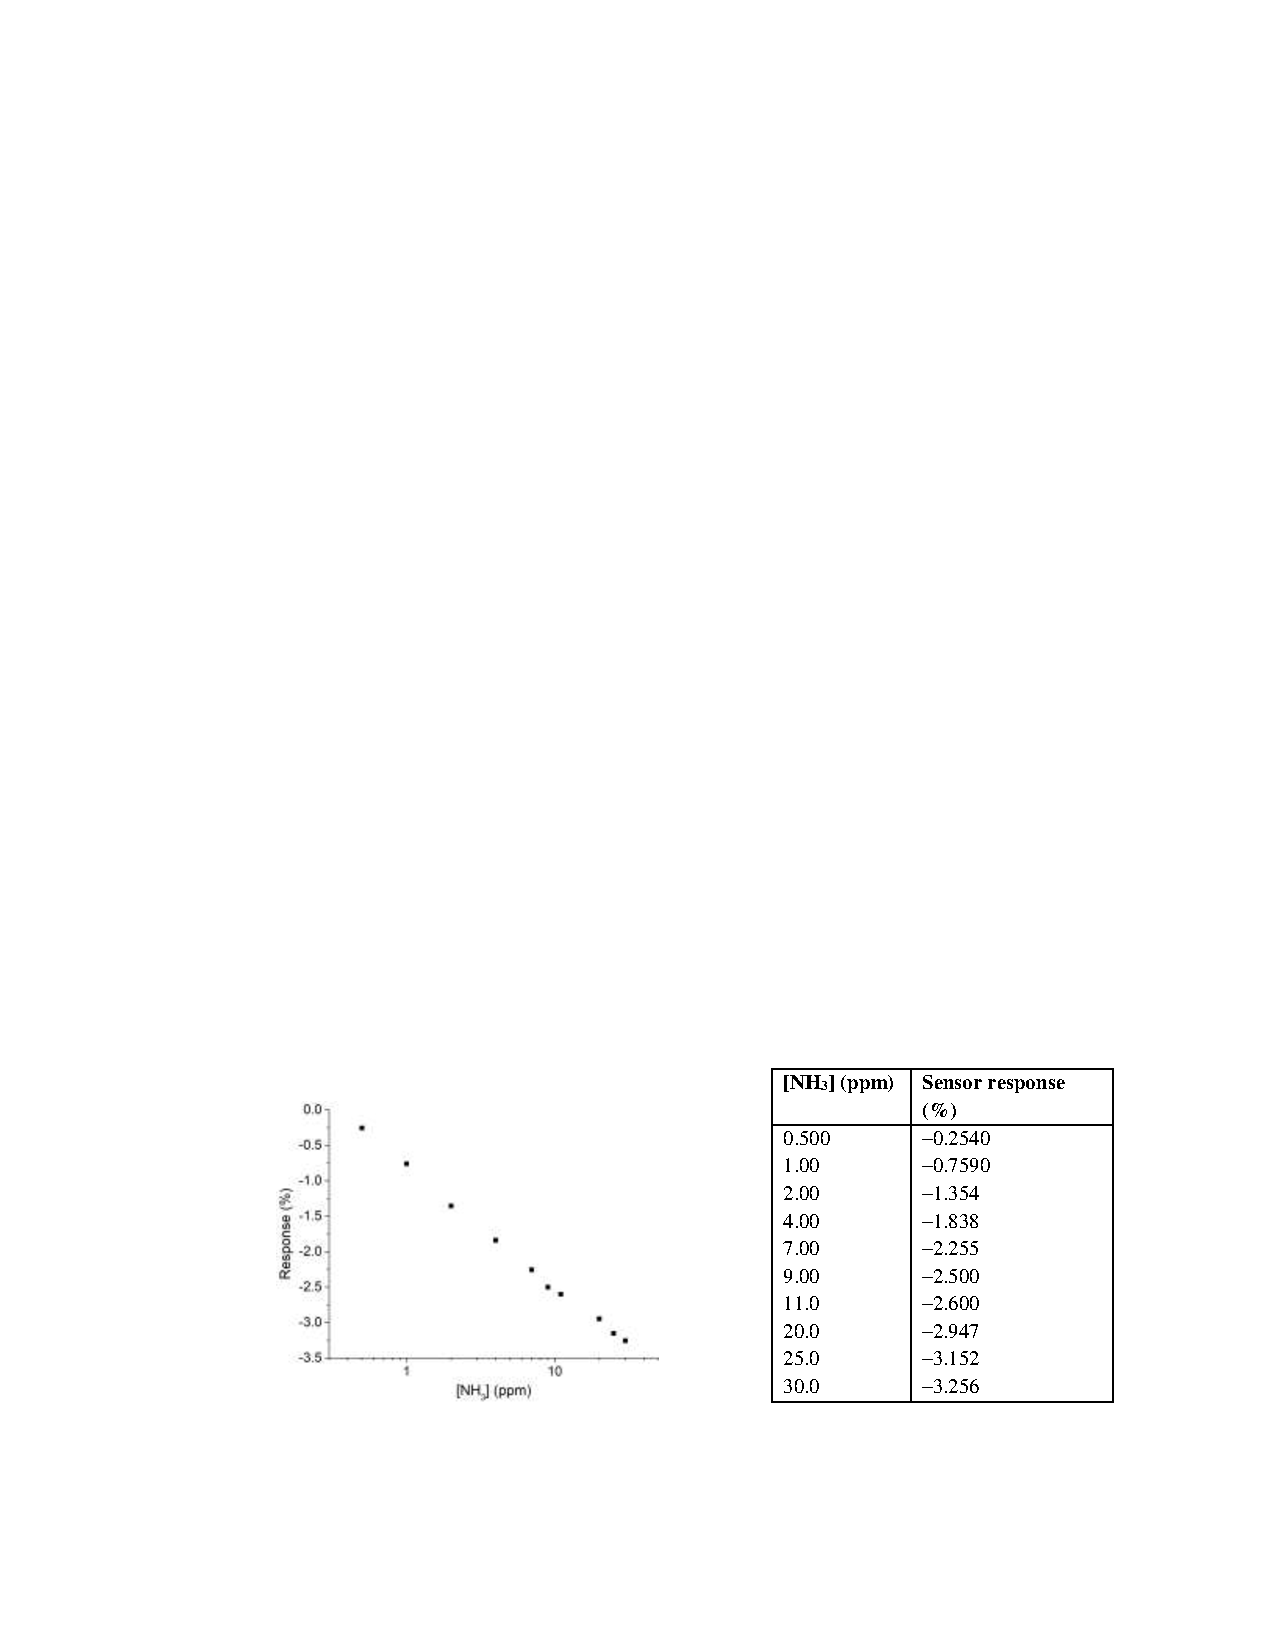
\includegraphics[width=14cm]{./pic/t11-4.pdf}
\end{figure}

\noindent\textbf{11.4.} 在探测器测得数据的线性区域作一条校准曲线,得到形如$y=a+bx$的校准曲线方程。

\noindent\textbf{11.5.}
用此探测器探测一肝脏疾病患者呼吸中的氨浓度,检测器检测到−3.812\%的信号变化。计算病人呼吸中的氨浓度。
